%!TEX program = xelatex

% \documentclass[notes]{beamer}
% \documentclass[notes=only]{beamer}
\documentclass{beamer}

% Good bibliography
\RequirePackage[backend=biber]{biblatex}
\addbibresource[datatype=bibtex]{biblio.bib}

% Icon Fonts
\RequirePackage{academicons}
\RequirePackage{fontawesome5}

% Correct the path when including svg pictures
\RequirePackage{import}

% For nice verbatim
\RequirePackage{minted}

% To resize graphic and table
\RequirePackage{graphics}

% For captions
\RequirePackage{caption}

% Arrange theme
\usetheme[
	progressbar=frametitle,
	sectionpage=none,
	numbering=fraction
]{metropolis}

% Color the progress:
% - SciLifeLabGreen for SciLifeLab
% - violet for KI
\definecolor{SciLifeLabGreen}{HTML}{95C11E}
\setbeamercolor{progress bar}{fg=SciLifeLabGreen,bg=white}

\title{Sarek and nf-core for Reproducibility}
\subtitle{SPHN Workflow Interoperability Workshop}
\titlegraphic{\vspace{1.9cm}
	\hfill
\includegraphics[height=.7cm]{pictures/SciLifeLab}%

	\hfill
\includegraphics[height=.7cm]{pictures/NGI}%

	\hfill\includegraphics[height=.7cm]{pictures/Barntumörbanken-logo}%
}

\author{\vspace{-.6cm}
	\faUser\ Maxime U. Garcia\\
	\faTwitter\ \href{https://twitter.com/gau/}{@gau}\\
	\faGithub\ \href{https://github.com/MaxUlysse/}{@MaxUlysse}\\
	\faGlobe\ \href{https://maxulysse.github.io/}{maxulysse.github.io}
	\vfill
}

\date{\vfill}

\begin{document}

{
	\usebackgroundtemplate{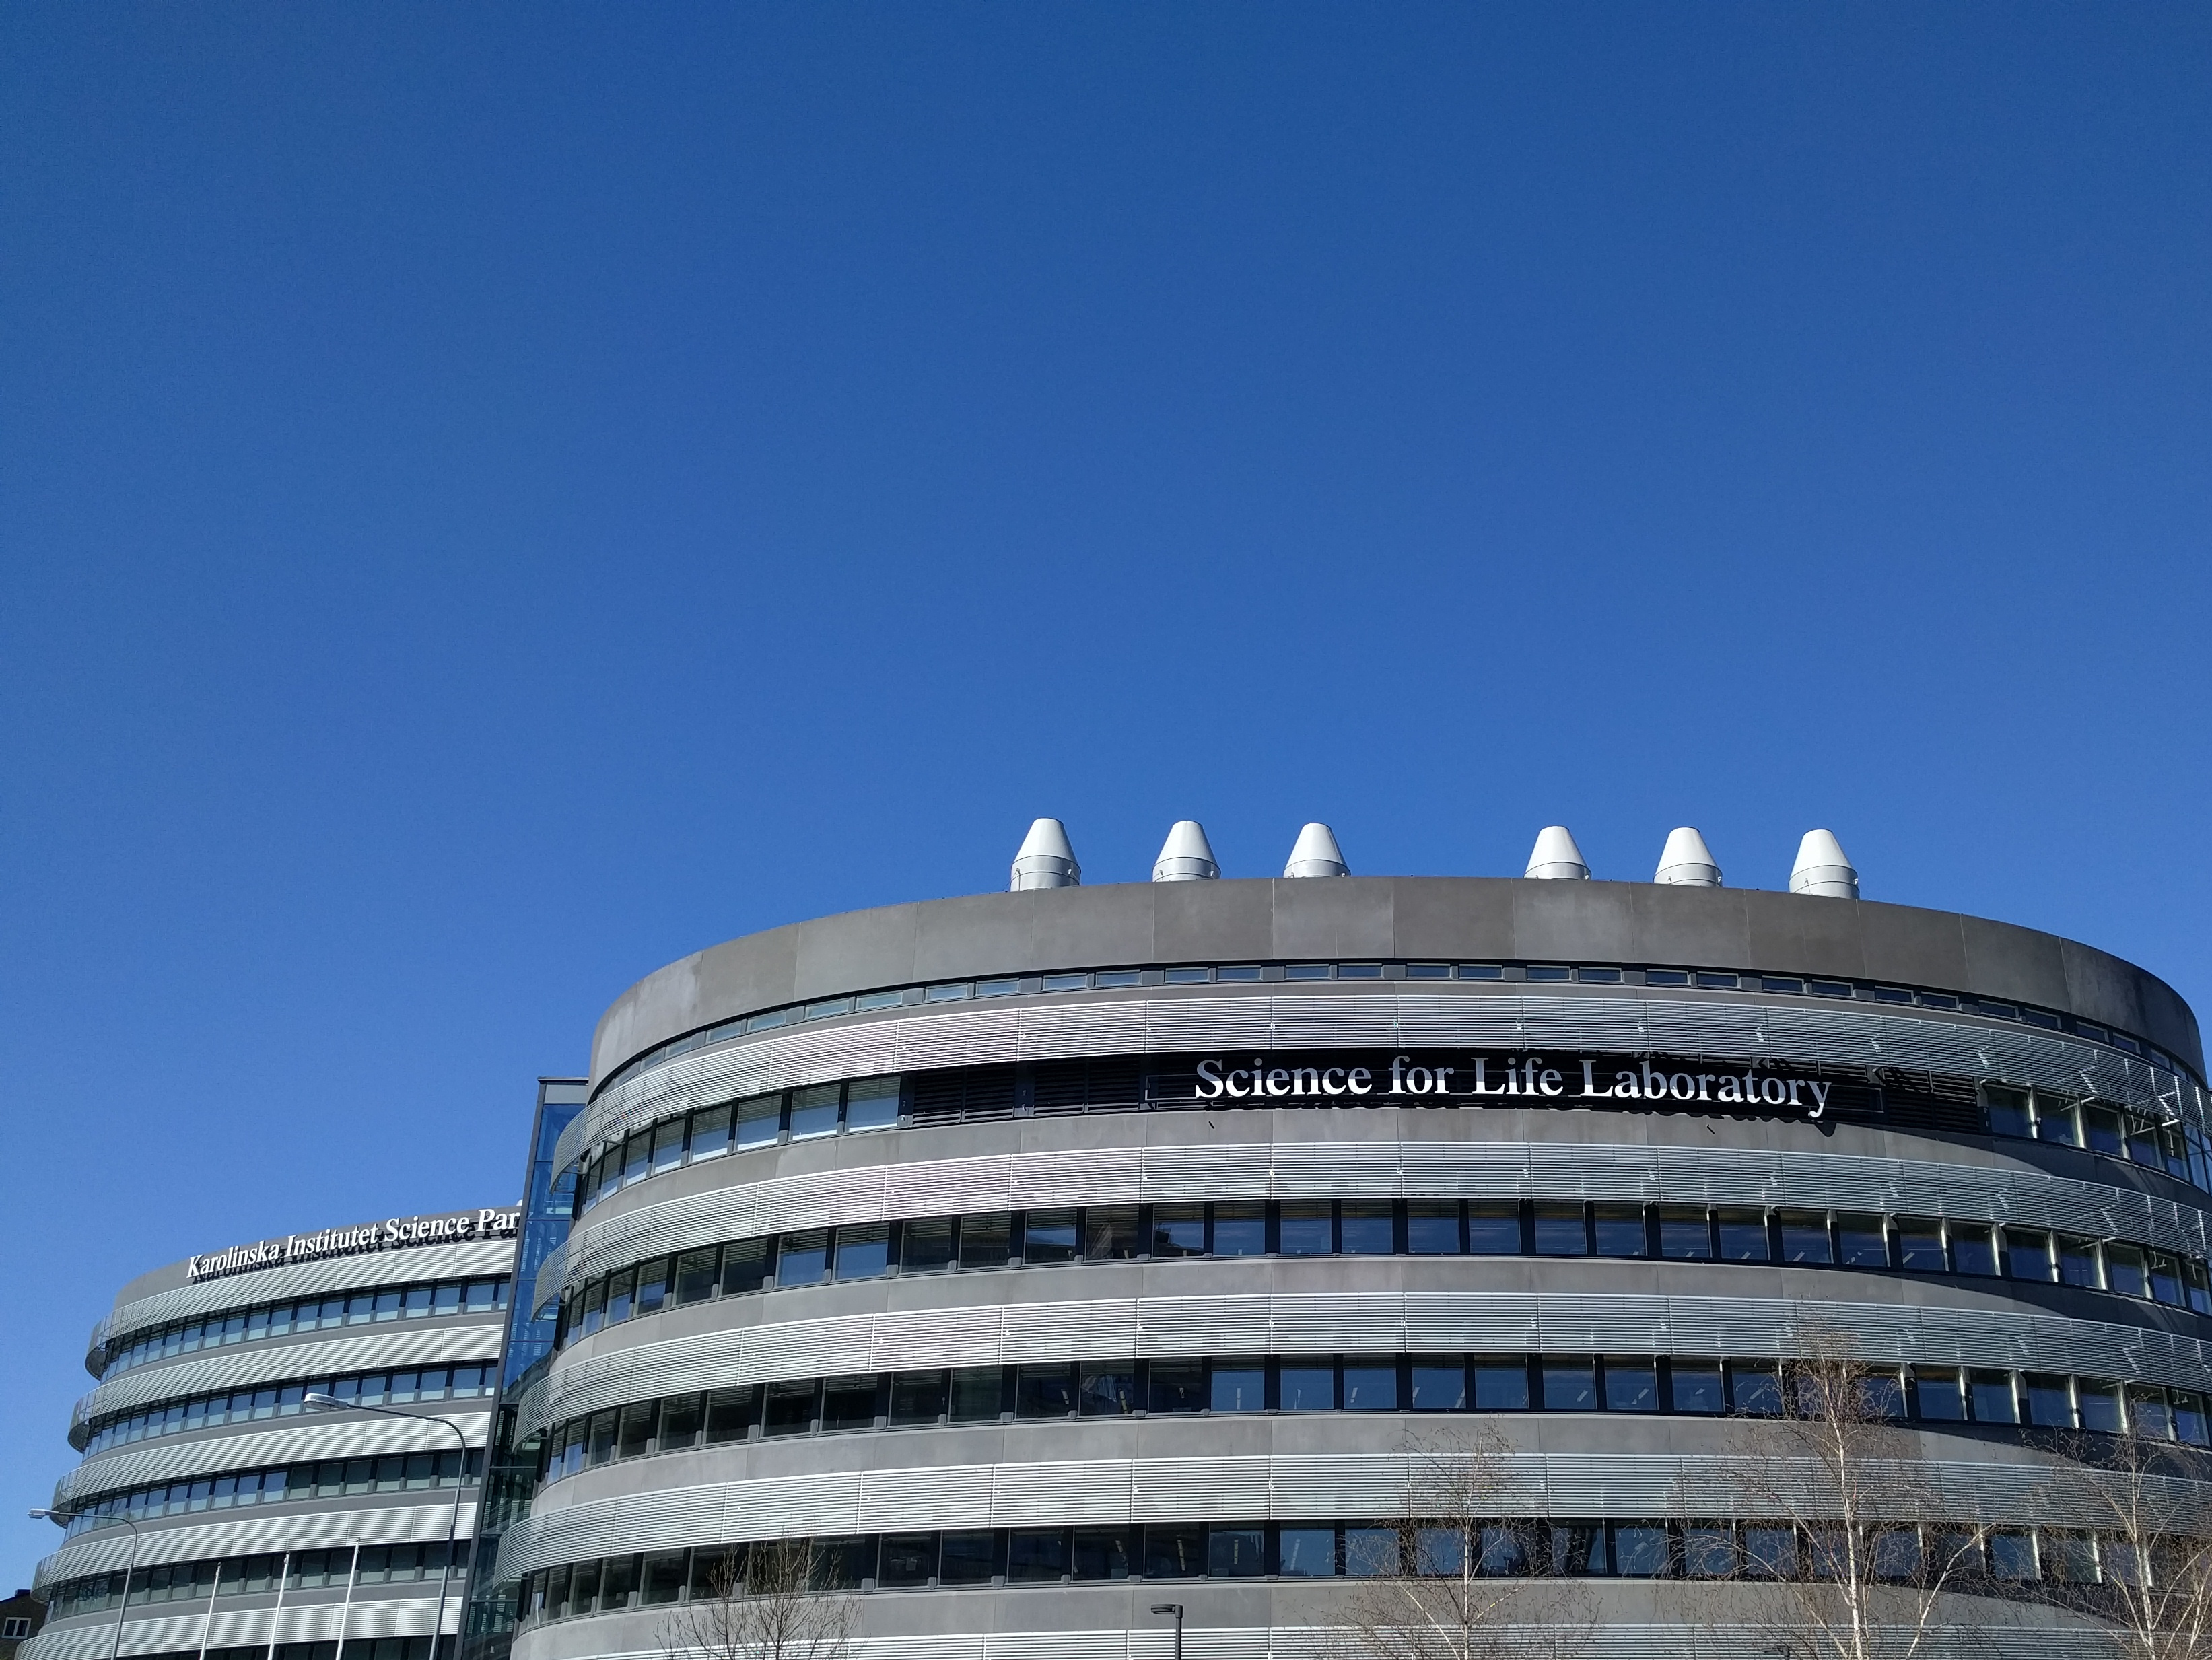
\includegraphics[width=\paperwidth]{pictures/SciLifelab-BlueSky2.jpg}}
	\setbeamercolor{normal text}{fg = white, bg = white}
	\maketitle
}

\section{ScilifeLab}

\begin{frame}{Science for Life Laboratory}
	\begin{figure}
		
\includegraphics[height=1.5cm]{pictures/SciLifeLab}
		\captionof*{figure}{\faGlobe\ \url{https://scilifelab.se/}}
	\end{figure}
	\only<1>{
		\centering SciLifeLab is a national centre for molecular biosciences\\with focus on health and environmental research

		\begin{figure}
			\hfill%
			
\includegraphics[height=1.5cm]{pictures/KI}%
			\hfill%
			
\includegraphics[height=1.5cm]{pictures/KTH}%
			\hfill%
			
\includegraphics[height=1.5cm]{pictures/SU}%
			\hfill%
			
\includegraphics[height=1.5cm]{pictures/UU}%
			\hfill%
			\hfill%
		\end{figure}
	}
	\only<2>{
		\centering Infrastructure Services

		\begin{table}
			\resizebox{.8\textwidth}{!}{%
			\begin{tabular}{lll}
				Genomics 						&	Proteomics								&	Metabolomics \\
														&														& \\
				Single Cell Biology	&	Bioimaging and Molecular	&	Chemical Biology and Genome \\
														&	 Structure								&	Engineering \\
														&														& \\
				Drug Discovery 			&	Diagnostics								&	Bioinformatics \\
			\end{tabular}}
		\end{table}
	}
\end{frame}

\section{NGI}

\begin{frame}{National Genomics Infrastructure}
	\begin{figure}
		
\includegraphics[height=1.5cm]{pictures/NGI}
		\captionof*{figure}{\faGlobe\ \url{https://ngisweden.scilifelab.se/}}
	\end{figure}
	\only<1>{
		Our mission is to offer a \textbf{state-of-the-art infrastructure} for massively parallel DNA sequencing and SNP genotyping, available to researchers all over Sweden.

		We provide \textbf{guidelines and support} for sample collection, study design, protocol selection and bioinformatics analysis.
	}
	\only<2>{
		\begin{figure}
			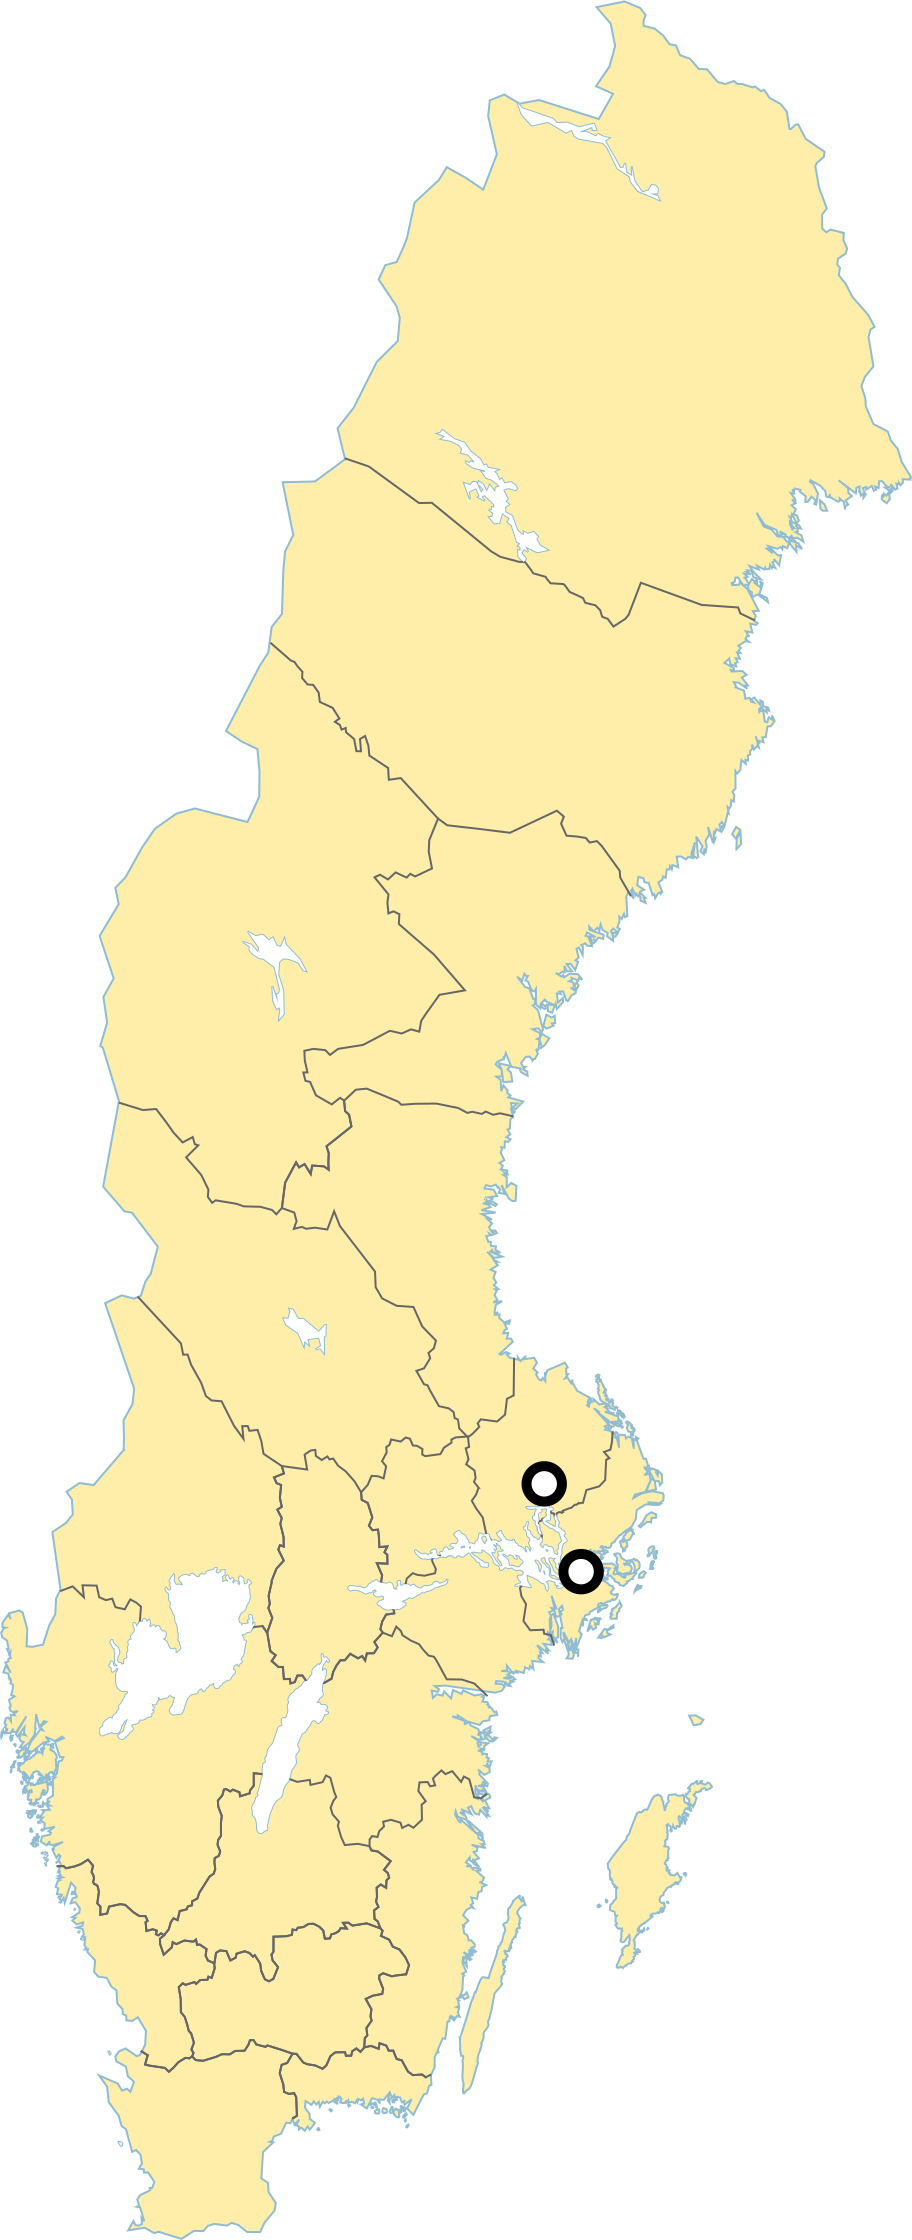
\includegraphics[height=4cm]{pictures/Sweden-map-NGI.png}
		\end{figure}
	}
\end{frame}

\begin{frame}{NGI Nodes}
	\begin{figure}
		
\includegraphics[height=1cm]{pictures/NGI}
		\captionof*{figure}{\faGlobe\ \url{https://ngisweden.scilifelab.se/}}
	\end{figure}
	\only<1>{\begin{itemize}
		\item Stockholm
		\item Uppsala
	\end{itemize}}
	\only<2>{\begin{itemize}
			\item Genomics Production - Genomics Applications Development
			\item SNP\&Seq - Uppsala Genome Center
	\end{itemize}}
\end{frame}

\begin{frame}{NGI Portal}
	\begin{figure}
		
\includegraphics[height=.7cm]{pictures/NGI}
		\captionof*{figure}{\faGlobe\ \url{https://ngisweden.scilifelab.se/}}
	\end{figure}
	\begin{figure}
		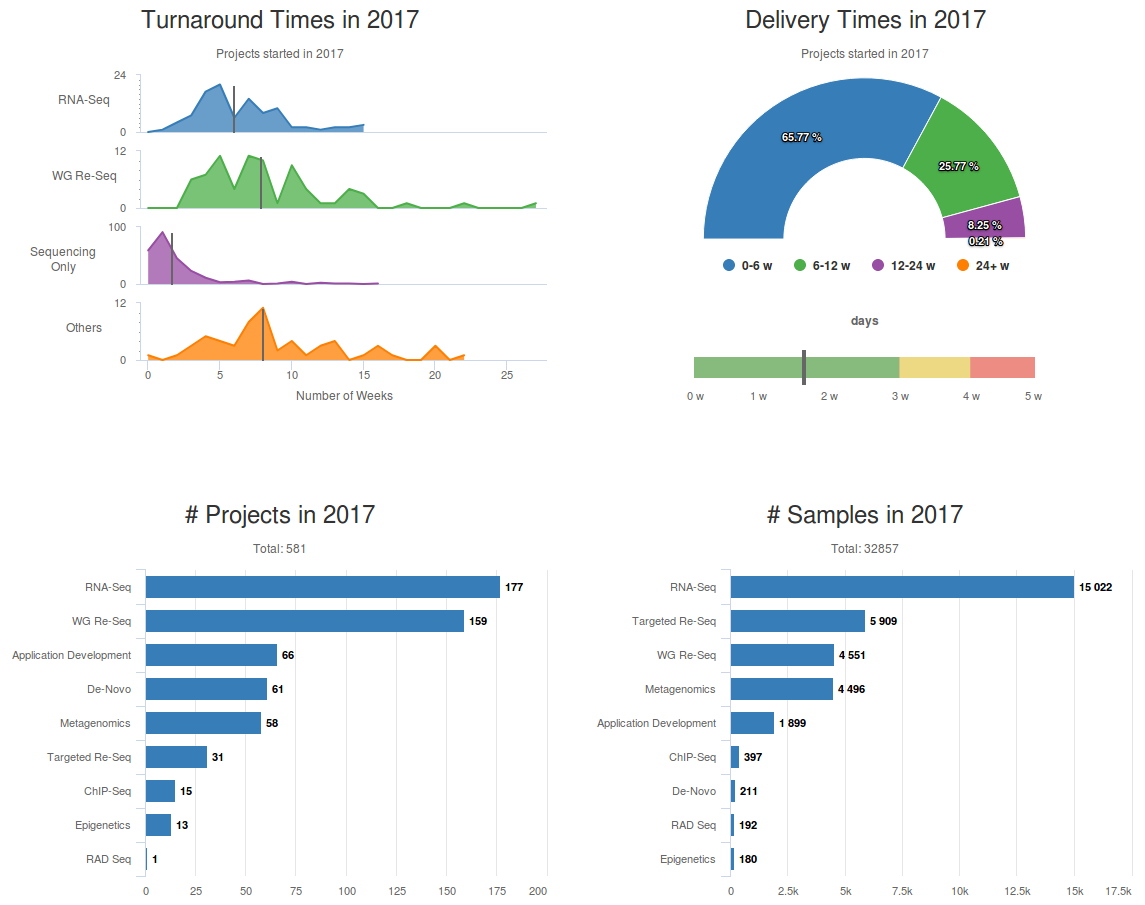
\includegraphics[height=6cm]{pictures/NGI-Portal.png}
	\end{figure}
\end{frame}

\section{NBIS}

\begin{frame}{National Bioinformatics Infrastructure Sweden}
	\begin{figure}
		
\includegraphics[height=.7cm]{pictures/NBIS}
		\captionof*{figure}{\faGlobe\ \url{https://www.nbis.se/}}
	\end{figure}
	\begin{figure}
		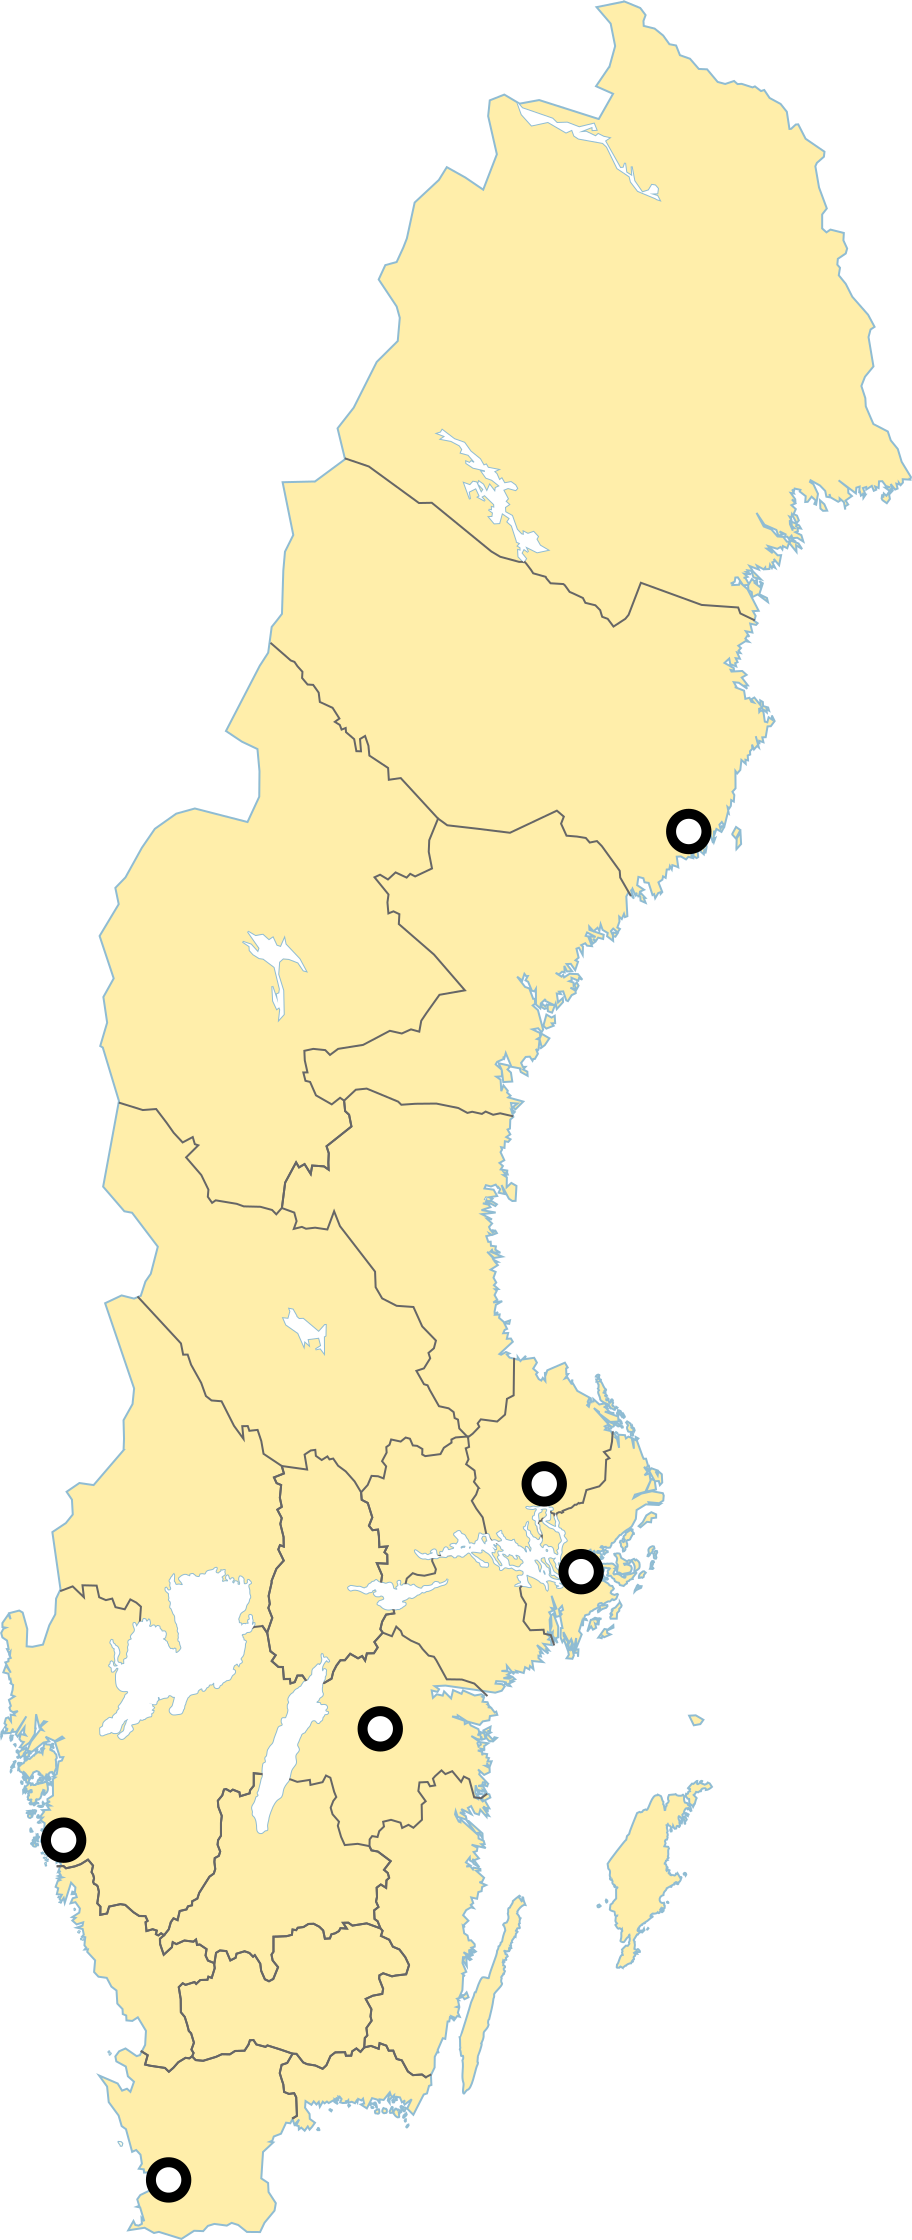
\includegraphics[height=4cm]{pictures/Sweden-map-NBIS.png}
	\end{figure}
	\begin{itemize}
		\item Distributed infrastructure
		\item Swedish node in ELIXIR
	\end{itemize}
\end{frame}

\section{Sarek}

\begin{frame}{Sarek}
	\begin{figure}
		
\includegraphics[height=7cm]{pictures/Sarek_discovery.jpg}
		\captionof*{figure}{James Frain as Sarek, "Star Trek: Discovery"}
	\end{figure}
\end{frame}

\begin{frame}{What is Sarek?}
	\vfill
	\begin{figure}
		
\includegraphics[height=1cm]{pictures/Sarek_no_border}
		\captionof*{figure}{\faGlobe\ \url{http://opensource.scilifelab.se/projects/sarek/}}
	\end{figure}
	\begin{itemize}
		\pause
		\item Nextflow pipeline
		\item<3-> Developed at NGI
		\item<4-> In collaboration with NBIS
		\item<5-> Support of The Swedish Pediatric Tumor Biobank
	\end{itemize}
	\begin{figure}
		
\includegraphics[height=1cm]{pictures/NGI}<3->
		\only<3->{\hfill}
		\includegraphics[height=1cm]{pictures/Barntumörbanken-logo}<5->
		\only<4->{\hfill}
		
\includegraphics[height=1cm]{pictures/NBIS}<4->
	\end{figure}
	\vfill
\end{frame}

\begin{frame}{Sarek is now in two flavors}
	\begin{figure}
		
\includegraphics[height=1cm]{pictures/Sarek}
	\end{figure}
	\pause
	\begin{figure}
		
\includegraphics[height=1cm]{pictures/Sarek_germline}
	\end{figure}
	\begin{figure}
		
\includegraphics[height=1cm]{pictures/Sarek_somatic}
	\end{figure}
\end{frame}

\begin{frame}{What does Sarek do?}
	\begin{figure}
		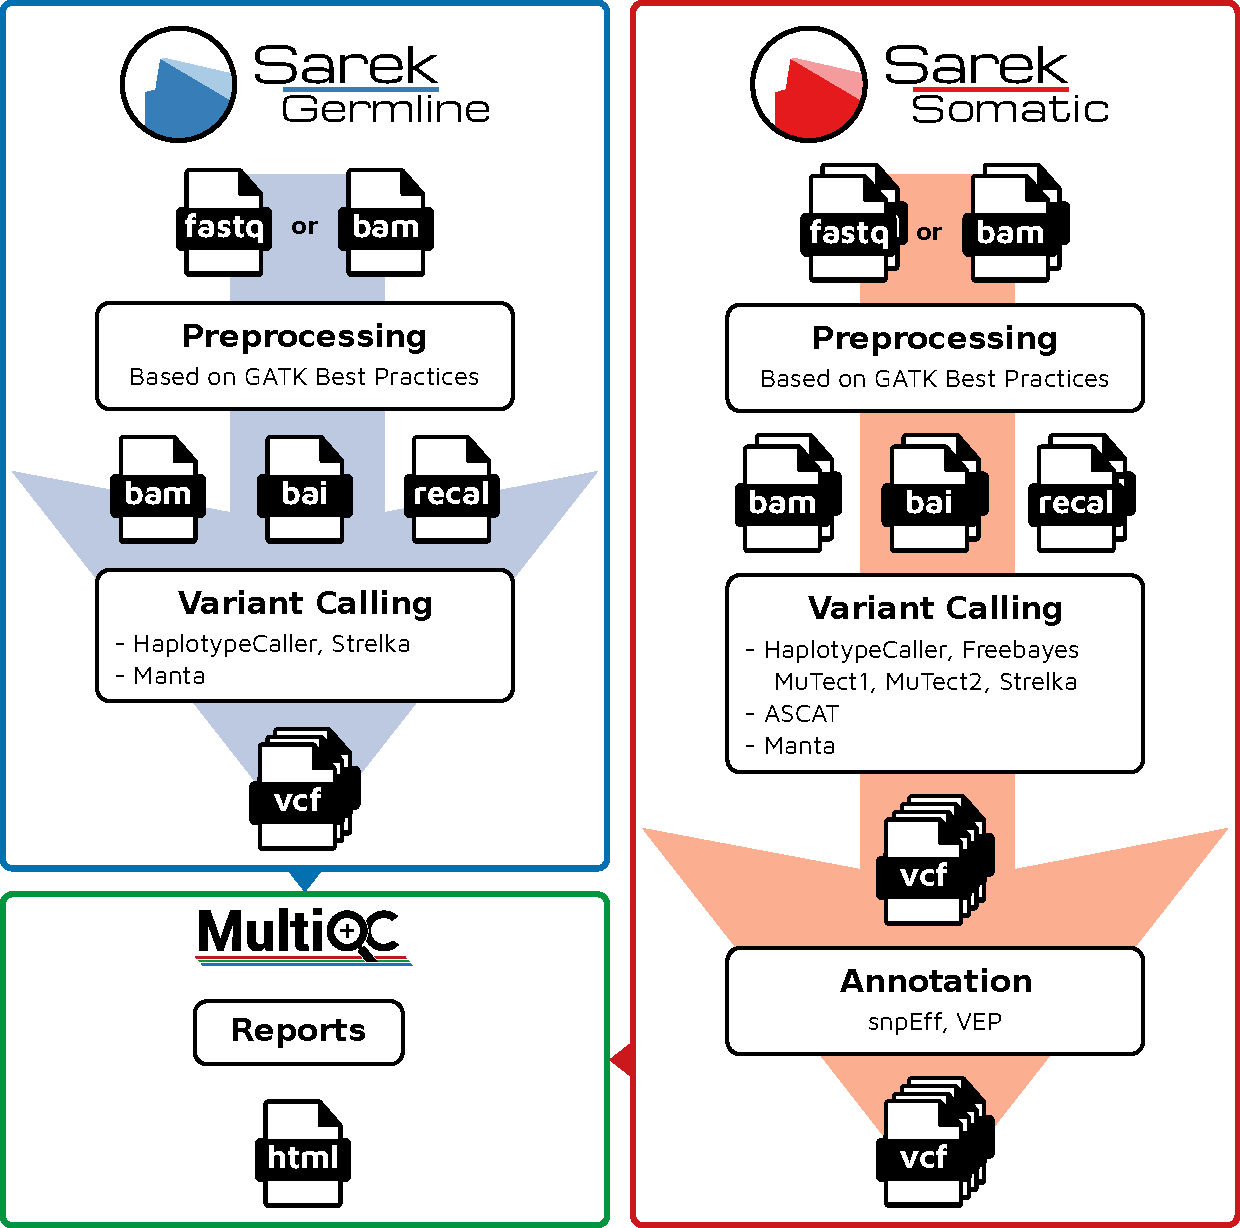
\includegraphics[height=7cm]{pictures/Sarek_workflow}
	\end{figure}
\end{frame}

\begin{frame}{What does Sarek do?}
	\begin{figure}
		
\includegraphics[height=1cm]{pictures/Sarek_no_border}
	\end{figure}
	\begin{itemize}
		\item WGS analysis (Tumor/Normal pair or Germline)
		\begin{itemize}
			\item FASTQ(s) to annotated VCF(s)
			\item Multiple entry points
		\end{itemize}
		\pause
		\item Handles both GRCh37, GRCh38 and custom genomes
		\pause
		\item Uses containers (Reproducibility, Portability)
		\begin{itemize}
			\item Docker or Singularity
		\end{itemize}
	\end{itemize}
\end{frame}

\section{Interoperability}

\begin{frame}{Where do I use Sarek?}
	\begin{itemize}
		\item My own Computer
		\pause
		\item UPPMAX - Irma - NGI Production Cluster
		\item UPPMAX - Rackham - Cluster
		\item UPPMAX - Bianca - Secure Cluster
		\pause
		\item Travis CI
		\pause
		\item AWS
	\end{itemize}
\end{frame}

\begin{frame}{Where can Sarek be used?}
	\begin{itemize}
		\item Any POSIX compatible system
	\end{itemize}
\end{frame}

\begin{frame}{Interoperability}
	\only<1-2>{\begin{itemize}
		\item Reproducibility
		\pause
		\item Portability
	\end{itemize}}
	\only<3>{\begin{itemize}
		\item Easy Reproducibility
		\item Easy Portability
	\end{itemize}}
\end{frame}

\section{nf-core}

\begin{frame}{NGI pipelines}
	\begin{figure}
		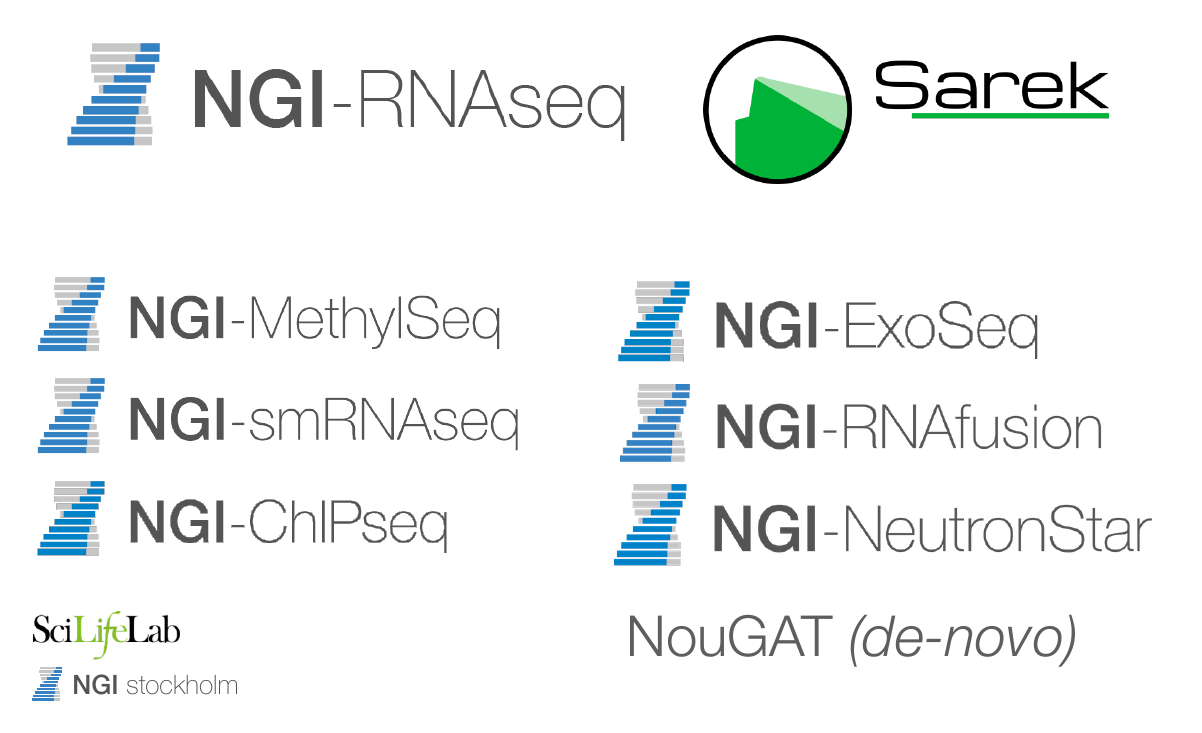
\includegraphics[height=6cm]{pictures/NGI-Pipelines.png}
	\end{figure}
\end{frame}

\begin{frame}{Who is using NGI pipelines?}
	\begin{figure}
		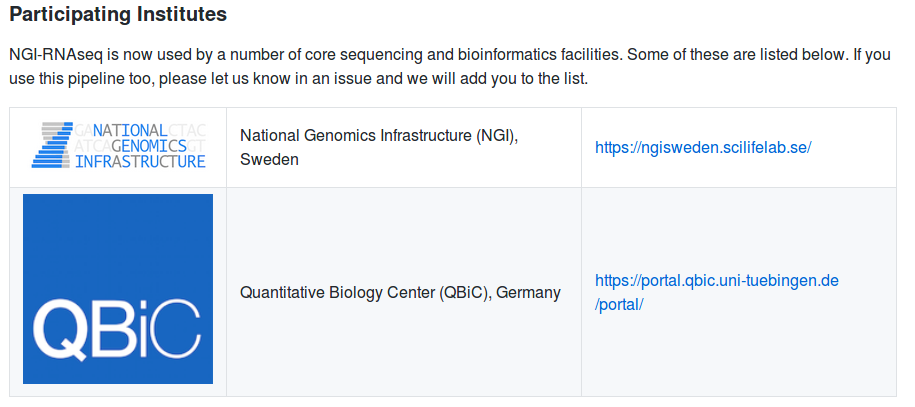
\includegraphics[height=5cm]{pictures/MultipleInstitutes.png}
	\end{figure}
\end{frame}

\begin{frame}{NGI-RNASeq}
	\faGlobe\ \url{https://github.com/SciLifeLab/NGI-RNAseq}
	\begin{figure}
		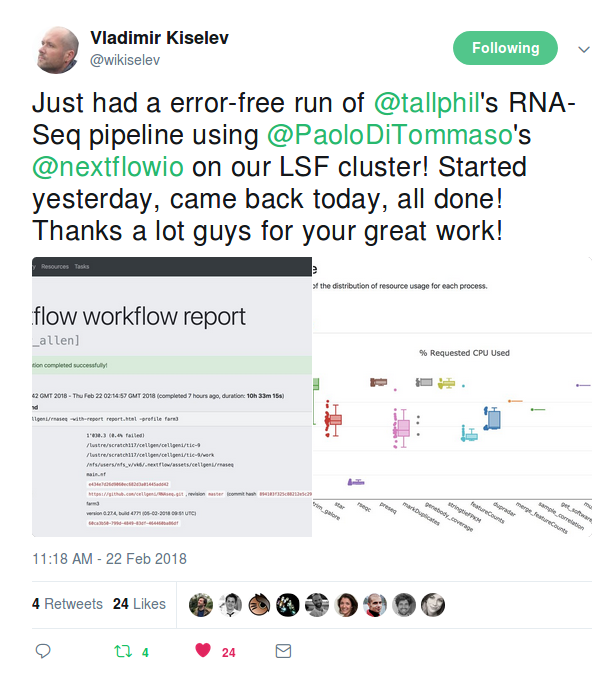
\includegraphics[height=6cm]{pictures/ErrorFreeRun.png}
	\end{figure}
\end{frame}

\begin{frame}{nf-core}
	\begin{figure}
		
\includegraphics[height=1cm]{pictures/nf-core}
		\captionof*{figure}{\faGlobe\ \url{https://nf-core.github.io/}}
	\end{figure}
	A community effort to collect a curated set of Nextflow analysis pipelines
	\begin{itemize}
		\item GitHub organisation to collect pipelines in one place
		\item No institute-specific branding
		\item Strict set of guideline requirements
		\item Automated testing for code style and function
	\end{itemize}
\end{frame}

\begin{frame}{A set of strict rules}
	\begin{figure}
		
\includegraphics[height=1cm]{pictures/nf-core}
		\captionof*{figure}{\faGlobe\ \url{https://nf-core.github.io/}}
	\end{figure}
	All Nextflow pipelines must have:
	\begin{itemize}
		\item MIT licence
		\item Software bundled using Containers
		\item Continuous Integration testing
		\item Stable release tags
		\item Common pipeline structure and usage
		\item Excellent documentation
	\end{itemize}
\end{frame}

\begin{frame}{NGI pipelines}
	\begin{figure}
		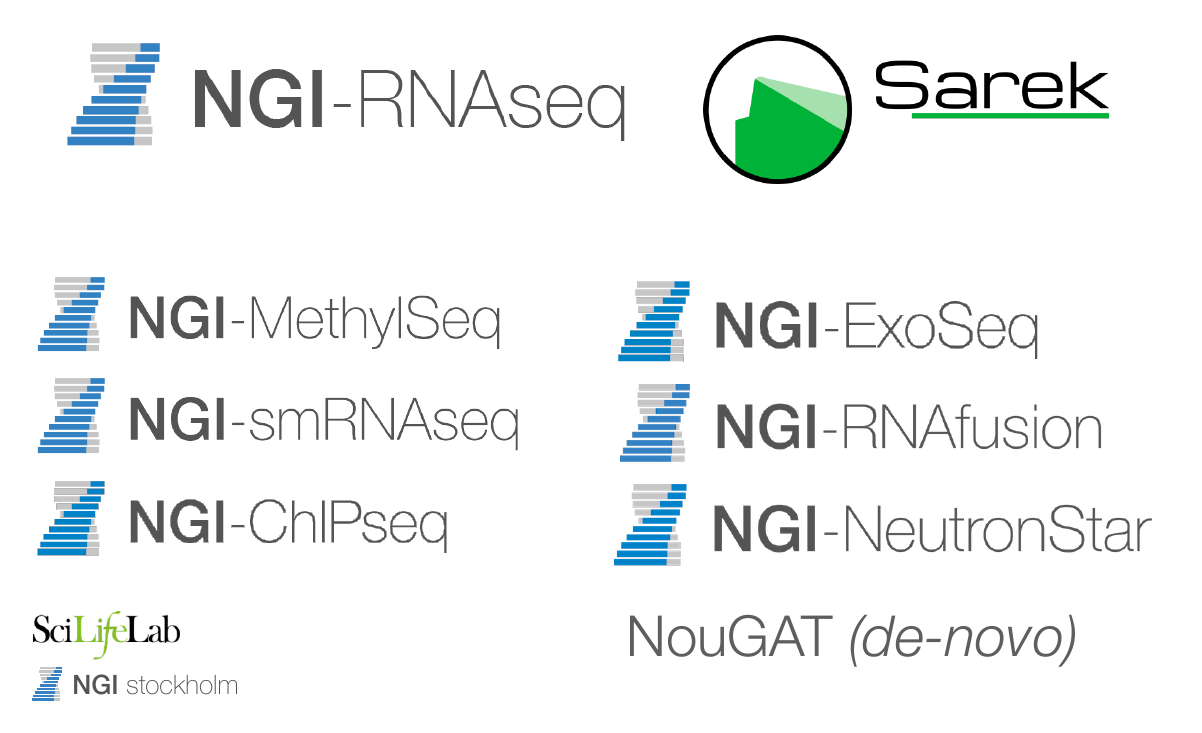
\includegraphics[height=6cm]{pictures/NGI-Pipelines.png}
	\end{figure}
\end{frame}

\begin{frame}{A first pipeline transfered}
	\begin{figure}
		
\includegraphics[height=1.2cm]{pictures/weHaveAPipeline.png}
	\end{figure}
	\begin{figure}
		
\includegraphics[height=3cm]{pictures/methylseq_logo}
		\captionof*{figure}{\faGlobe\ \url{https://github.com/nf-core/methylseq}}
	\end{figure}
\end{frame}

\section{Acknowledgments}

\begin{frame}{The List of People Involved}
	\begin{figure}
		
\includegraphics[height=1cm]{pictures/Sarek}
	\end{figure}
	\begin{table}
		\resizebox{.8\textwidth}{!}{%
		\begin{tabular}{ll}
			Sebastian DiLorenzo &	Markus Mayrhofer \\
			Jesper Eisfeldt 		&	Monica Nistèr \\
			Phil Ewels					& Björn Nystedt \\
			Maxime Garcia 			&	Pall Olason \\
			Szilveszter Juhos 	&	Markus Ringnér \\
			Max Käller 					&	Pelin Sahlén \\
			Malin Larsson 			&	Johanna Sandgren \\
			Marcel Martin 			&	Teresita Díaz De Ståhl \\
		\end{tabular}}
	\end{table}
\end{frame}

\begin{frame}{The List of People Involved}
	\begin{figure}
		
\includegraphics[height=1cm]{pictures/nf-core}
	\end{figure}
	\only<1>{
		\begin{itemize}
			\item The National Genomics Infrastructure (NGI), SciLifeLab, Stockholm, Sweden
			\item The Quantitative Biology Center (QBiC), Universität Tübingen, Germany
			\item The Genomics Institute of Singapore (GIS), A*STAR, Singapore
		\end{itemize}
	}

	\only<2>{
		\begin{table}
			\resizebox{.8\textwidth}{!}{%
			\begin{tabular}{ll}
				Chih Chuan				& Denis Moreno \\
				Paolo Di Tommaso	& Remi-Andre Olsen \\
				Phil Ewels				& Senthilkumar Panneerselvam \\
				Sven Filinger			& Alexander Peltzer \\
				Maxime Garcia			& Chuan Wang \\
				Rickard Hammarén	& Andreas Wilm \\
			\end{tabular}}
		\end{table}
	}
\end{frame}

\begin{frame}{Get involved!}
	\begin{itemize}
		\item We have gitter channels

		\faGitter\ \url{https://gitter.im/SciLifeLab/Sarek}

		\faGitter\ \url{https://gitter.im/nf-core/Lobby}
		\pause
	\end{itemize}
	\begin{itemize}
		\item Our code is hosted on Github

		\faGithub\ \url{https://github.com/SciLifeLab/Sarek}

		\faGithub\ \url{https://github.com/nf-core}
	\end{itemize}
\end{frame}

{
	\usebackgroundtemplate{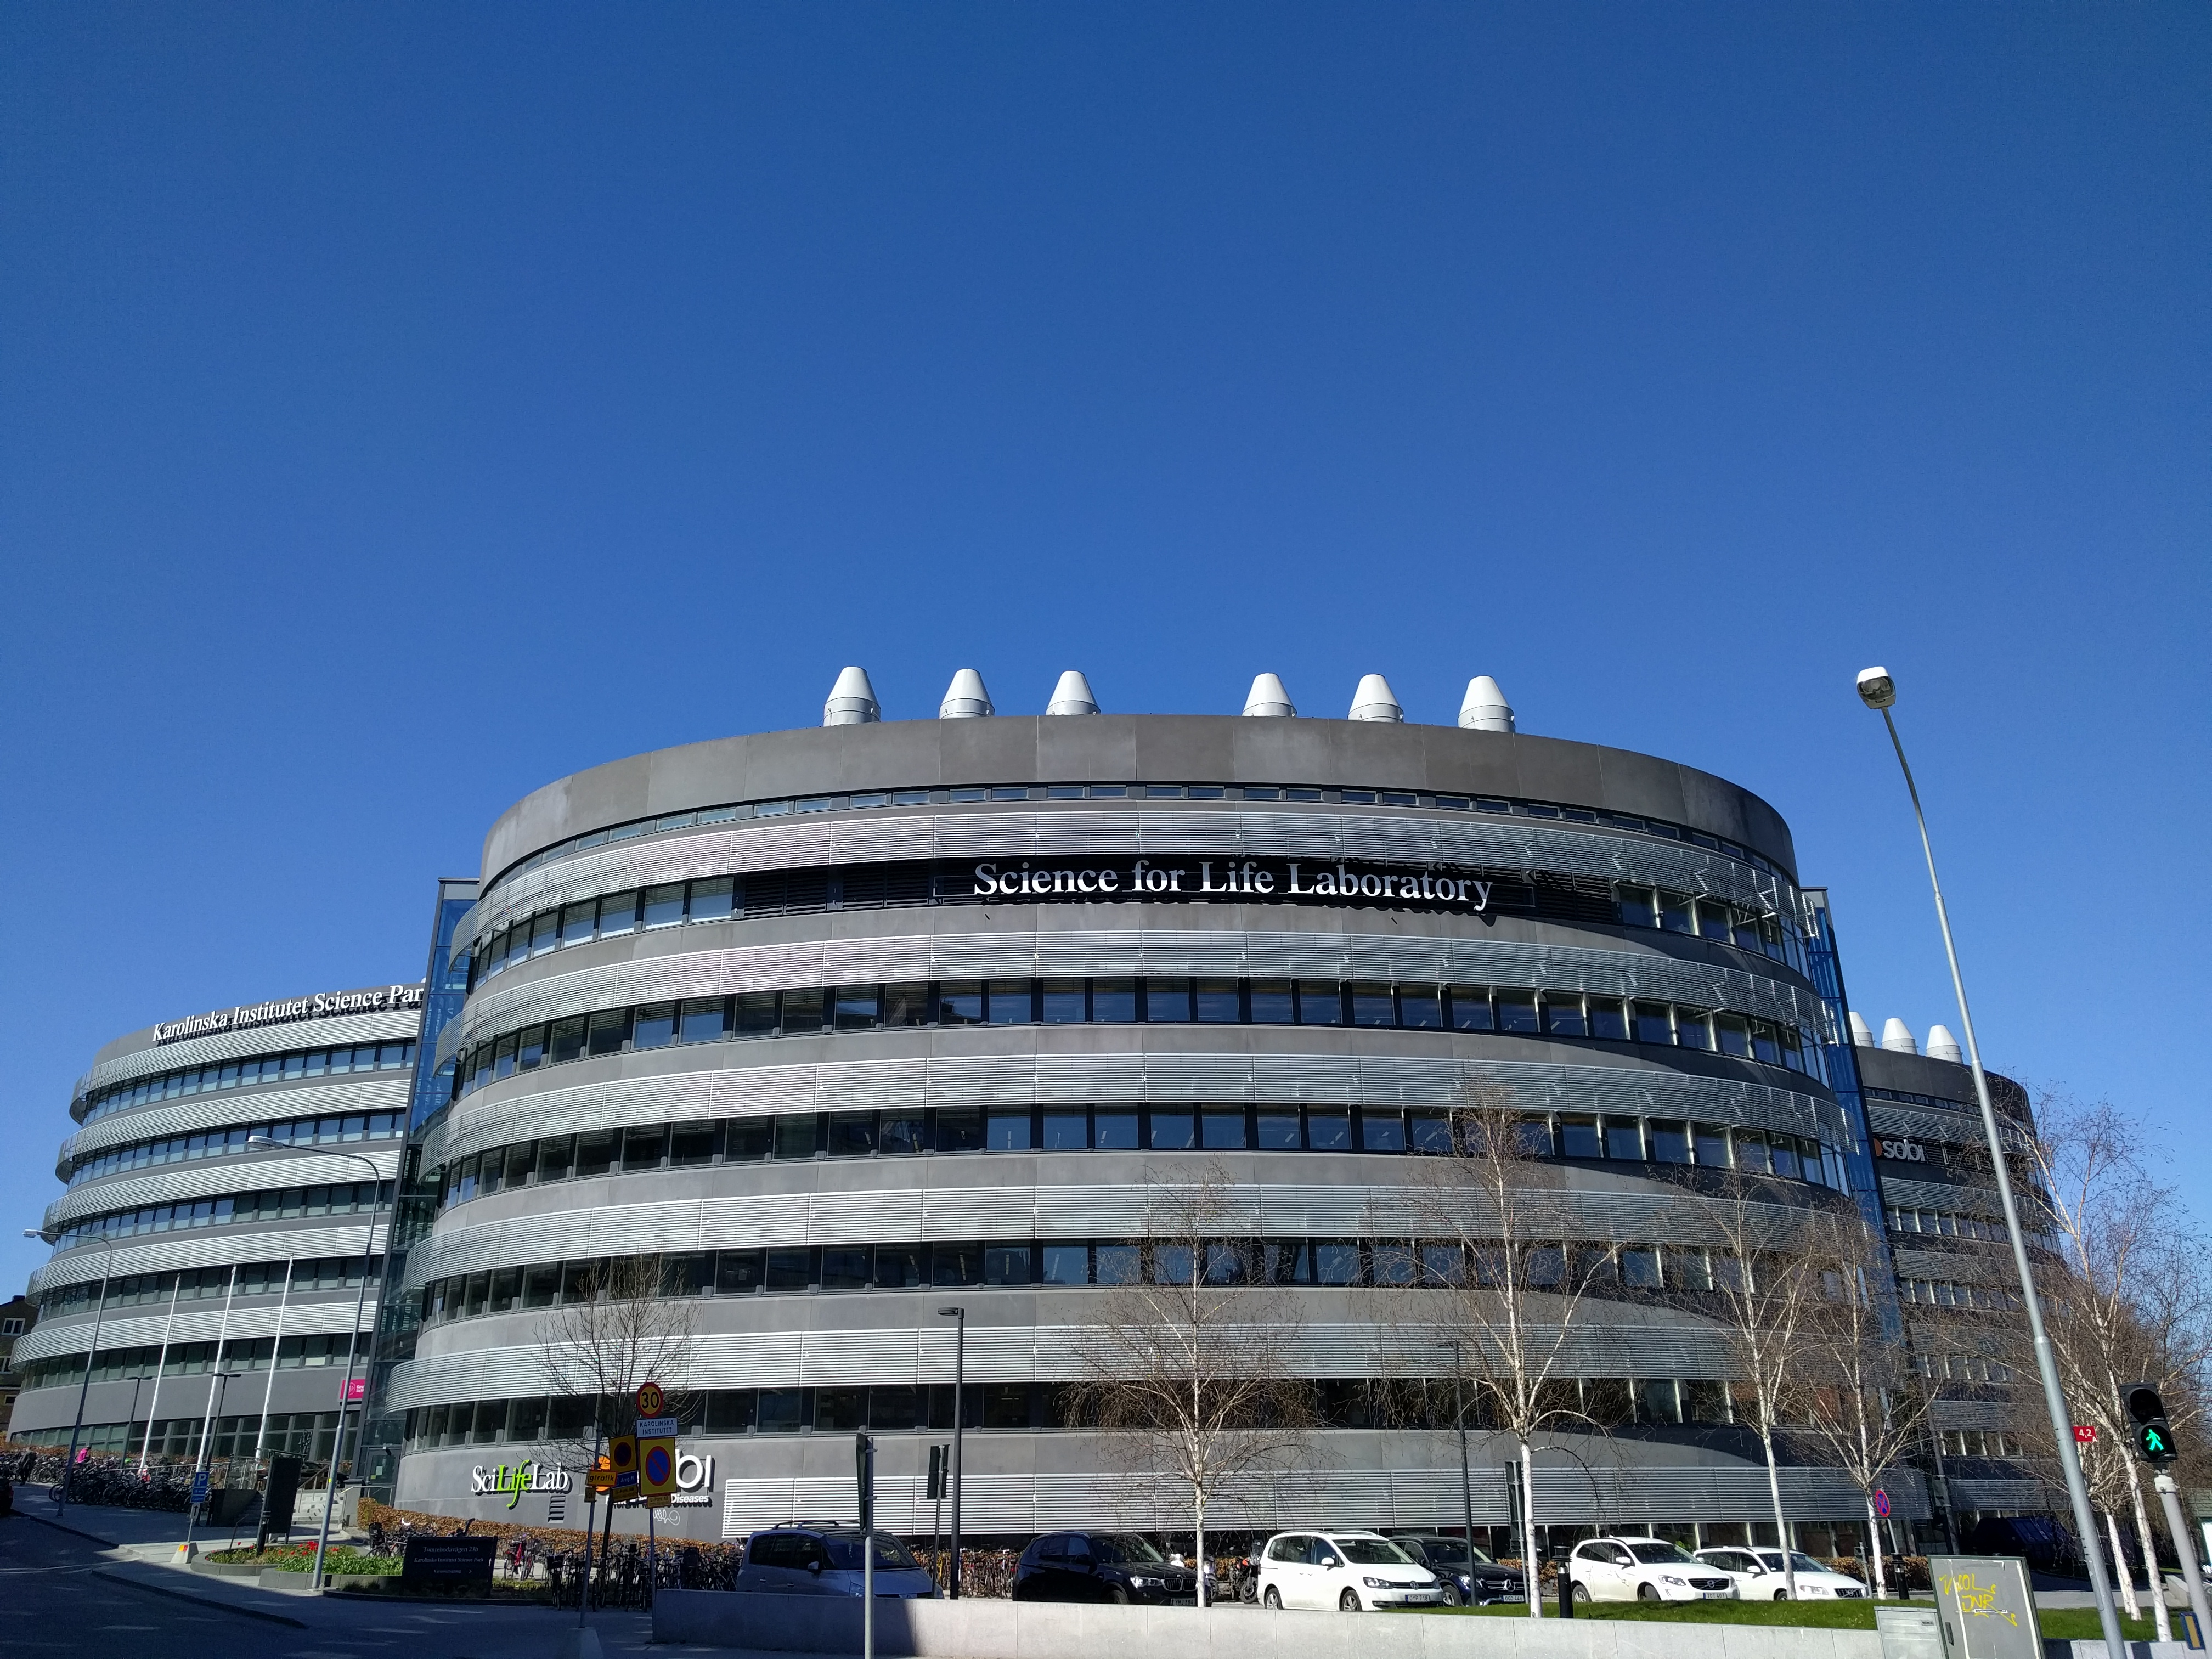
\includegraphics[width=\paperwidth]{pictures/SciLifelab-BlueSky.jpg}}
	\begin{frame}[plain,noframenumbering]{Any questions?}
	\end{frame}
}

\end{document}
